%%This is a very basic article template.
%%There is just one section and two subsections.
\documentclass[12pt]{article}
\usepackage[margin=1in]{geometry}
\begin{document}
%%To do:
%%___________________
%%  fill in data numbers
%%  sources
%%  explain normalization
%%  more equations in methods (only if we need to fill space)
%%  numbers for paring
%%  numbers for normalization

\section{Problem}
``What should I do when I'm bored?''  is a question that almost everyone has
asked at one time. A brief look at common Google searches highlights the demand
for activity ideas. We started this project to be able to answer this question
for our users. The only information that should be required from a user is 
a number of ratings of other businesses. Using only that information we want to
be able to give a predicted rating for any other business. We should also be
able to give a user a list of their highest predicted ratings as a good answer
to ``what should I do?''. Additionally we would like to give a user some insight
into why we are recommending a business. This will help to give confidence in
our recommendations, and will also give the user some expectation of what to
expect when they arrive at the business.

A running instance of our solution can be found at http://zoufbox.
Note, you must access this from within the CS department.

\newcommand{\bestRMSE}{0.9307 }
\newcommand{\bestK}{48 }
\newcommand{\bestNetflixRMSE}{0.8712 }
\newcommand{\netDiff}{0.06 }

\newcommand{\numBusCA}{707 } 
\newcommand{\numBusTotal}{2,452 }

\newcommand{\numRatingCA}{8,970 } 
\newcommand{\numRatingTotal}{28,310 }

\section{Data}
We acquired the academic dataset from yelp. The rating consists of ?? users and
?? businesses. The businesses are all located in the vicinity of $30$ different
universities in the United States. There are a total of ?? ratings. We initially
misunderstood the datasets. We thought we were obtaining two different
datasets, one from Michigan and one from Princeton, but we actually recieved the
entire dataset twice. Our initial plan was to get two different datasets,
training on the first then finally testing on the second. Unfortunately we
unknowingly trained on the entire body of data, so we weren't able to test on
any fresh data. 

For our application, this isn't as big of a problem as others in practice. This
is because in practice, we will be able to tune the model on the entire body of
data fairly often. Because of our optimizations, tests run fairly quickly making
it possible to adjust the model fairly often. Keeping a set of fresh data to
test on is important for situations where you wish to have a solution that will
work on all datasets without any need for tuning and that really isn't our goal.

\section{Methods}
\subsection{Collaborative Filtering}

To give predicted ratings we decided to use a form of \emph{Collaborative
Filtering} (CF). CF techniques use the tastes of a large collection of users to
predict the taste of a single user.

A very simple example of collaborative filtering would be to use a method such
as difference squared to measure the distance between the ratings of any two
users. Once we have defined our distance function, if we want to predict a
rating of user $b$ on business $b$ we can do the following: Find the distance
between $u$ and each user with a rating for $b$, choosing the user $v$ with the
shortest distance to $u$. Now we say that since $u$ and $v$ usually have very
similar ratings, $u$ will probably feel the same about $b$ as $v$ does. This is
a very na\"{i}ve method, that can be improved by things like taking more related
users into account and averaging their rating for $b$.

Even with improvements to the previous method, we wouldn't really take the way
people make decisions about businesses into account. It won't be terribly
accurate, and there are a number of situations in which this method won't be
able to get a rating at all. If none of the users related to a user have a
rating for a business we wish to predict for, this simple CF algorithm will be
unable to make any prediction for that business at all. 

\subsection{Singular Value Decomposition}
To correct for these problems we decided to perform a matrix factorization
using singular value decomposition (SVD)\cite{bellkor}. SVD fixes both of the
problems that are mentioned above. It decomposes relationships between users
and businesses into some number of factors that influence the relationship.
This allows SVD to better model why people like particular businesses.
SVD can also use less direct relationships between users, so even if
closely related users don't have a rating for a business, we can still give a
prediction for it.

The goal of SVD is to decompose the given matrix $M$ into
matrices $P$ and $Q$ such that $P \times Q \approx M $. This means that if
matrix $M$ has dimensions $u \times b$, $P$ should be $u \times K$ and $Q$
should be $K \times b$. We know that $b$ and $u$ should be the number of
businesses and users respectively, but what is $K$? In SVD $K$ corresponds to
the number of \emph{latent factors} we believe determine the relationship
between users and businesses.

The only input to the SVD algorithm is a matrix $M$ of size $b \times u$ and the
integer $K$. The output of SVD is then matrices $P$ and $Q$. $P$ contains a
relationship between every user and every latent factor. Similarly $Q$ describes
relationships between businesses and latent factors. These relationships aren't
on the same scale as the input ratings of $M$, but they are relative. A value
of $.9$ between a user and a factor suggests that that user has a stronger
relationship to the factor than a value of $.4$. It is also possible to have a
negative relationship. Because $P \times Q$ is an
approximation for $M$, $P_u \cdot Q_b$ approximates a rating for user $u$ on
business $b$. This is referred to as Standard SVD\cite{bellkor}.

SVD on sparse matrices is calculated using an iterative gradient descent
approach to discover good values for $P$ and $Q$. Using gradient descent allows
us to calculate $P$ and $Q$ using only the observed values and ignoring any
empty values. This means that we initialize $P$ and $Q$ to some values, and
then calculate the distance from $P \times Q$ to $M$. We then move the values
in $P$ and $Q$ in the correct direction to decrease the distance. 
This means that the value of $P \times Q$ should move closer
to $M$ with each iteration. At the end of each iteration we measure the
difference between the previous distance and the current one. When we make a
small enough change, or a predetermined amount of iterations have occurred, the algorithm terminates.

Our goal in each iteration is given some $P$ and $Q$, for every $i$ and $j$ for
which there exists a rating $M_{ij}$ and for every latent variable $k$ from
$0\ldots K$, we should determine a new $P_{ik}$ and $Q_{kj}$. We do this using the
following equations

\[
\begin{array}{c}
P'_{ik}=P_{ik} + \alpha(E_{ij}Q_{kj}-\beta P_{ik}) \\
Q'_{kj}=Q_{kj} + \alpha(E_{ij}P_{ik}-\beta Q_{kj})
\end{array}
\]

\noindent where $E$ is the error between $P \times Q$ and the actual value.
What we are doing here is modifying each user and business association in a
direction that decreases the distance between $M$ and $P \times Q$. The term
multiplied by $\beta$ is the regularization term. This term keeps the values
from changing too quickly relative to how large they already are. This
restricts the absolute values in $P$ and $Q$ from growing too large to avoid
over-fitting the data.

You can see that each iteration is controlled by two additional parameters.
$\alpha$ scales the amount that we increase or decrease the values in $P$ and
$Q$. A larger $\alpha$ can lead to faster convergence, but if $\alpha$ gets too
big, it is possible that we will greatly overshoot the answer and simply
oscillate around it without ever reaching convergence. Similarly, if $\alpha$
is too small, the algorithm will reach convergence much slower than it would
with a more appropriate value for $\alpha$. We also use $\beta$ to control the
effect of our regularization term.  A larger $\beta$ will decrease the chance
of over-fitting but make convergence slower.

\subsubsection{Normalization}

Our ratings data comes from a 5-star system, which everyone can treat slightly
differently. For example, perhaps some users are particularly harsh and rarely
give out 5-star ratings, or others are particularly kind and rarely give any
business less than 3-stars. To account for this we normalize our data by
considering each rating to be comprised of four factors (cf. \cite{bellkor}): 

\begin{description}

  \item[Global Baseline] This is the global average of all ratings on the site
and serves as a baseline for all ratings.

  \item[User Specific] This is the different between the global average and
this users average, and serves to account for the users particular bias.

  \item[Business Specific] Same as \textbf{User Specific}, but for the business

  \item[User-Business Interaction] This is the specific interaction between this
user and this business. This is the term that we try to identify through SVD. 

\end{description}

By attempting to specifically identify the user-business interaction, we remove
the bias in the system, with the users, and with the businesses to more
accurately predict the user's rating of the business. 

\subsubsection{Capping}

People typically reserve the highest and lowest ratings for the perfect and
worst possible business respectively. Currently, a particularly strong factor
could give a very strong positive rating, such as $+7$, and a second factor has
a minor negative influence, such as $-1$, would result in an overall rating of
$+5$. That is, the high positive rating would negate any effects the small
negative rating would have. Thus, we cap the amount of influence each factor
can have on the rating to between $-5$ and $+5$ during the dot-product calculation
in our algorithm. With the cap in place, our
strong $+7$ rating is capped at $+5$ which allows the $-1$ rating to pull our
overall rating away from a perfect score and down to $+4$. \cite{funk}

\subsection{Framework}

Because we actually want to build a usable system on top of our recommendation
engine, we built a prototype website in Django\cite{django}. Django is an MVC
(Model-View-Controller) web framework based on Python. MVC frameworks like
Django provide modularity between the design and functionality of websites
along with convenient abstractions for accessing databases.  Behind the scenes,
a MySQL database is used to hold information about users, businesses, and
ratings.

\subsection{Challenges}

Our initial implementation had two problems: it used a dense matrix
representation, and it was implemented in Python. Because the gradient descent
algorithm only operates on non-zero ratings (we use zero ratings to represent
no rating), a dense matrix representation was extremely expensive, both in
memory and computationally. Because most of the ratings are zeroes, our first
large performance improvement came from switching to a sparse representation.
Instead of creating a 2-dimensional array containing a rating for every
user-business pair, we created a 1-dimensional array where each cell contained a
username, a business name, and a rating. This allowed us to use only a fraction
of the memory, and to save a large number of wasted loop iterations. The dense
matrix representation took up too much memory and completely stalled the program
in the setup stages, so we can't accurately analyze the speedup we got by
switching to a sparse representation.

The next step we took to improve performance was to move our algorithm code into
C++. To do this we used the Boost library to compile C++ code into a python
plug-in. Once this was done we could call our C++ code as if it were python code.
This gave a significant speedup and got us to the point where we could execute
tests in a reasonable amount of time. To improve the speed of tests even more we
implemented task-level parallelism, allowing us to run tests for different
values of $K$ simultaneously.

%In future work, we will look into parallelizing
%the algorithm code. This is an interesting challenge, because the outer loop
%appears to carry dependences. We suspect, however, that the order we update
%cells in $P$ and $Q$ actually won't have any effect on the correctness of the
%algorithm. This is easy to check because the distance should get better at every
%step. As long as that invariant holds, we can be sure our algorithm will
%eventually give a good answer.
%
%The dataset presented some challenges as well. The first challenge we dealt with
%is that some users and businesses had a very limited number of reviews. Users
%and Business with only a single review don't add any information to the
%algorithm, so we removed those. We also added a method for removing users and
%businesses with fewer than an arbitrary number of reviews. The effect of this is
%shown in the results section.


\section{Evaluation}
We evaluated our technique in phases. First, we generated data that
validates the correctness of the model, then we evaluated a small portion of
the dataset, and finally evaluated on the full dataset.

\subsection{Generated Data}
The core algorithm relies on finding a $P$ and $Q$ matrix that relate users and
businesses to latent factors (the columns of $P$ and $Q$).  Figuring out
specifically how a user $u$ feels about a business $b$ is just a matter of
taking the dot product of $P_u$ and $Q_b$.  Therefore, we started evaluation by
randomly generating a $P$ and $Q$ matrix, and then creating the rating table
by multiplying the matrices. Running our algorithm on this data yielded similar
$P$ and $Q$ matrices, which indicated that the algorithm was (fundamentally) doing
what we expected it to do.

\subsection{Real Data}
However, using generated data shows nothing about the validity of our model. In
order to show just how effective our model is, we needed to evaluate on
the actual businesses data from Yelp. We started evaluation by taking dense
chunks of data from the Yelp set. Thus, we'd only have a couple of thousand
ratings (instead of hundreds of thousands).  This step was critical to expose
inefficiencies in our calculations (indeed, once we started doing this, we
immediately realized the need to switch our code from Python to a C++ module).

For training, we removed California's businesses ratings from the Yelp data
set. This meant removing roughly \numBusCA businesses from \numBusTotal total
businesses and \numRatingCA from \numRatingTotal ratings.
The red line in Figure~\ref{fig:nocal} shows a plot of RMSE vs. K for all data excluding
California's. For the evaluation step, we ran our algorithm on ratings for
California businesses only. The red line in Figure~\ref{fig:cal} shows a plot of RMSE vs. K for
ratings only on California businesses. No parameters were changed between the
training and evaluation run. The graphs show that the K-values have roughly the
same effect on RMSE in both cases. Thus, a K-value that gives a good RMSE value
in the data excluding California gives a good RMSE value in the data for
California (and vice versa). This result indicates that our model works well on
data which we did not train or tune with. This also indicates that it might be
possible to make assumptions about the number of factors people use when
deciding what businesses they like. Because of this, it might be possible to
pick a K that gives good results across most realistic datasets.

\begin{figure}[ht!]
	\centering
	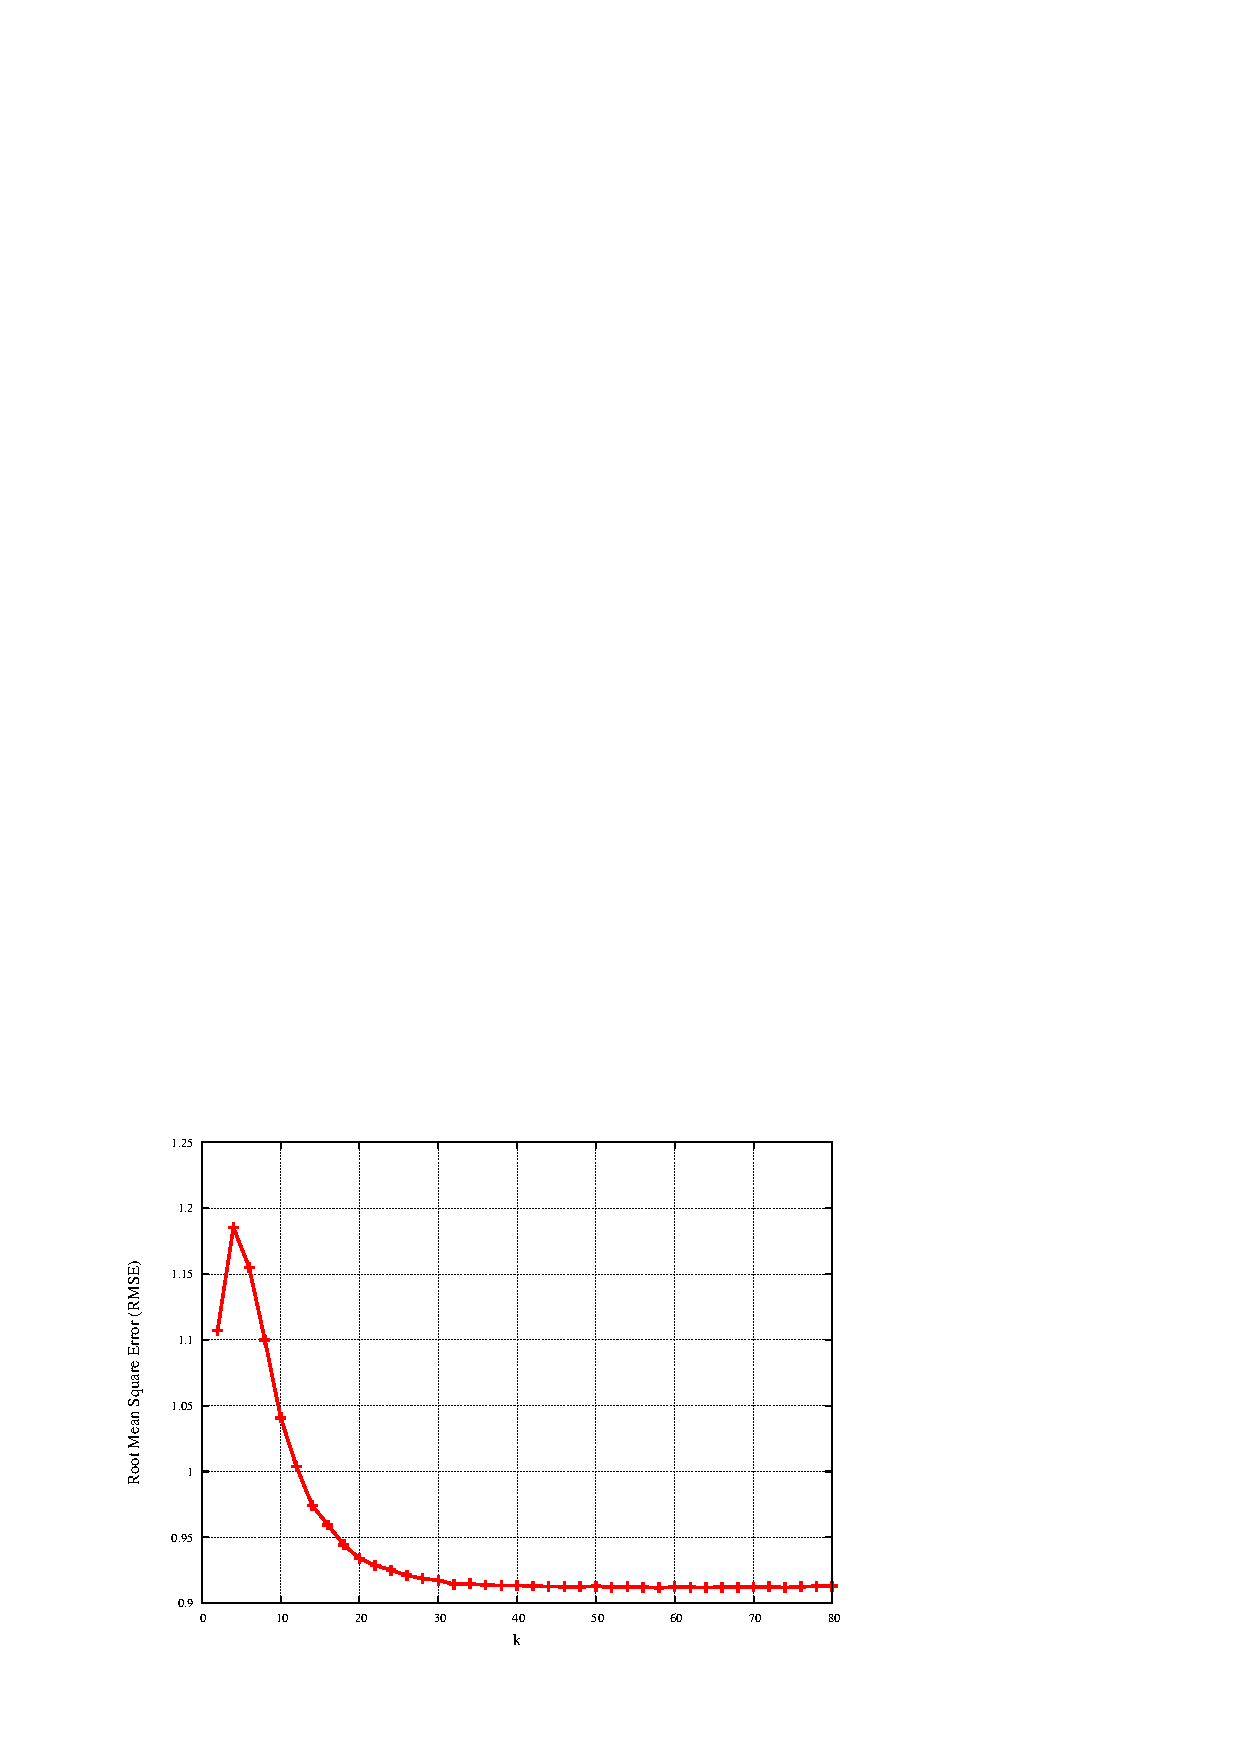
\includegraphics[scale=0.5]{figures/nocal.pdf}
	\caption[]{A plot of RMSE vs. K on our test set (all ratings excluding California businesses). Blue indicates our RMSE values when we did not use normalization; red uses normalization.}
	\label{fig:nocal}
\end{figure}


\begin{figure}[ht!]
	\centering
	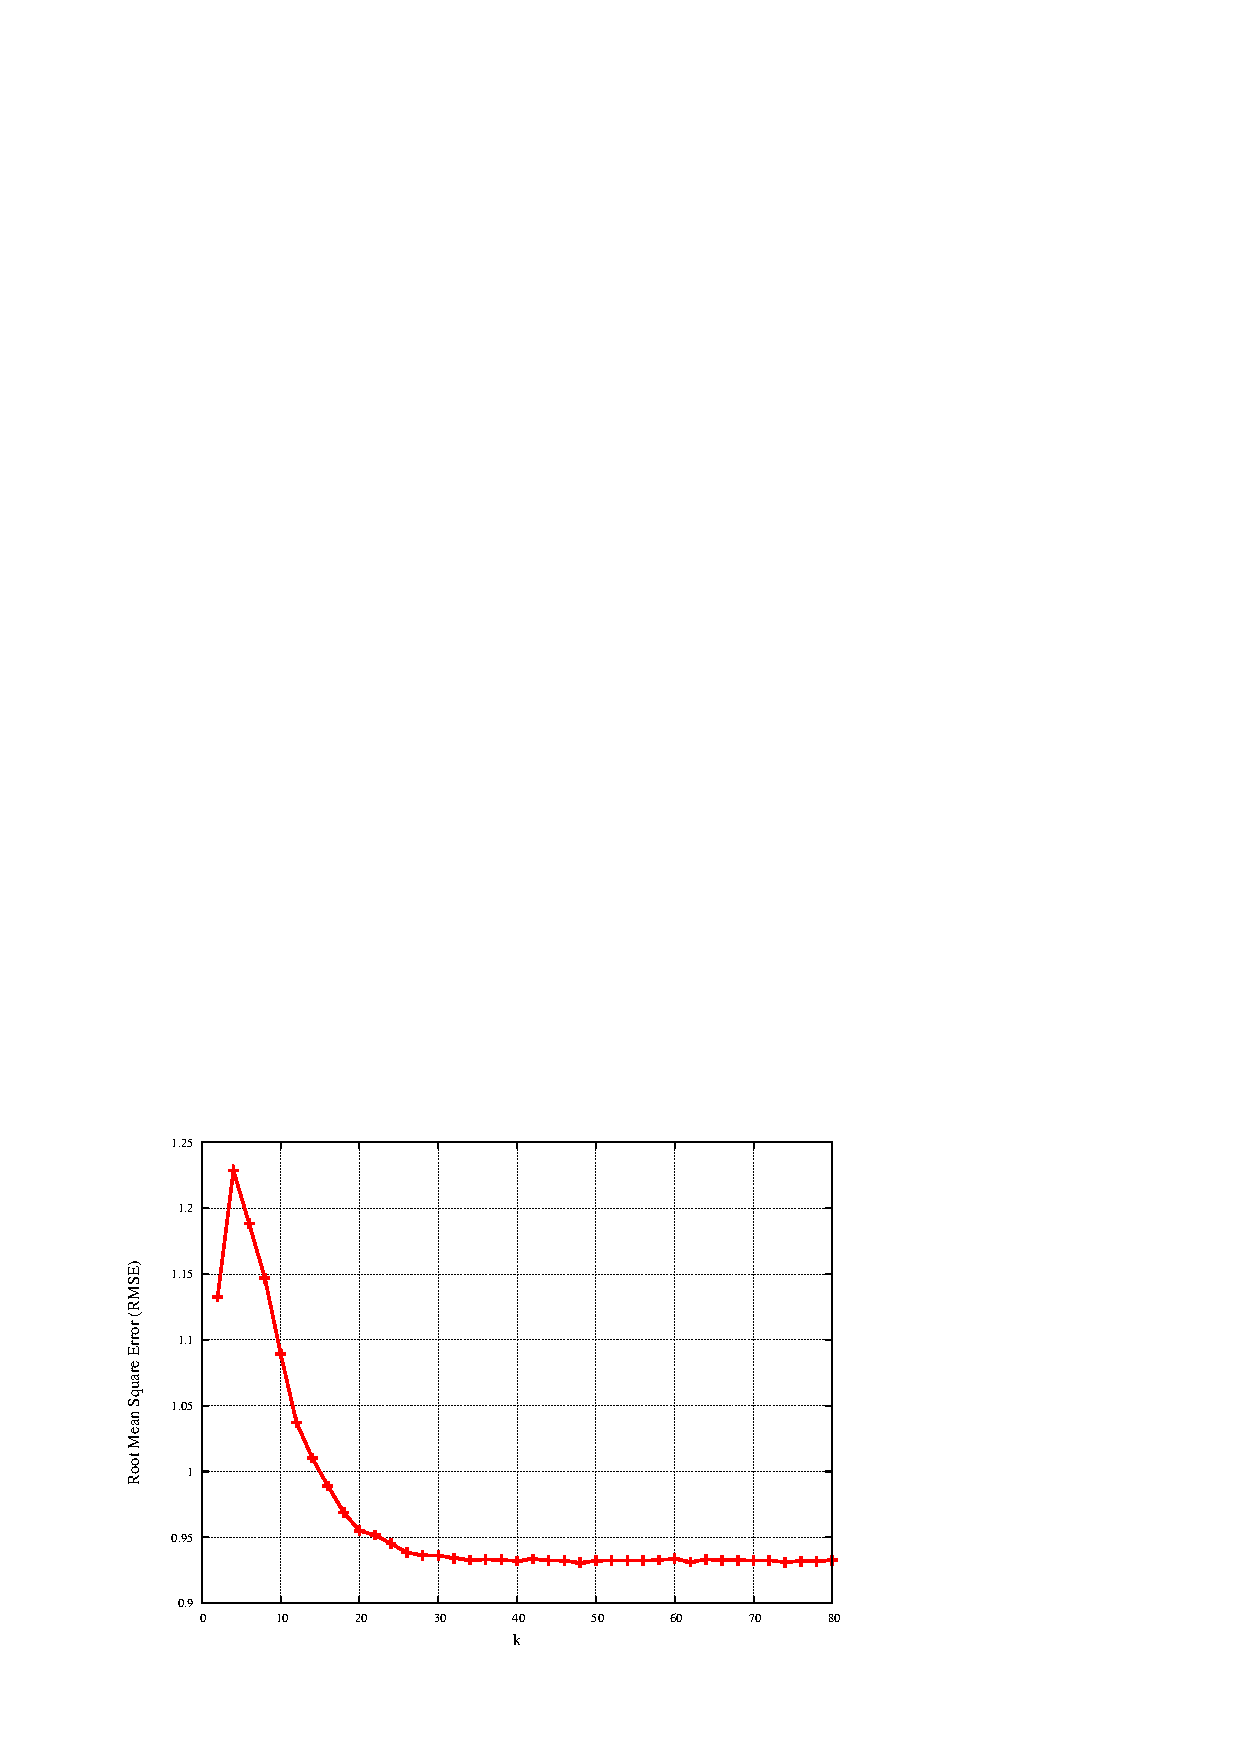
\includegraphics[scale=0.5]{figures/cal.pdf}
	\caption[]{A plot of RMSE vs. K on our evaluation set. Red indicates ratings on all California businesses and green indicates food-related business ratings in California}
	\label{fig:cal}
\end{figure}

%\begin{figure}[ht!]
%	\centering
%	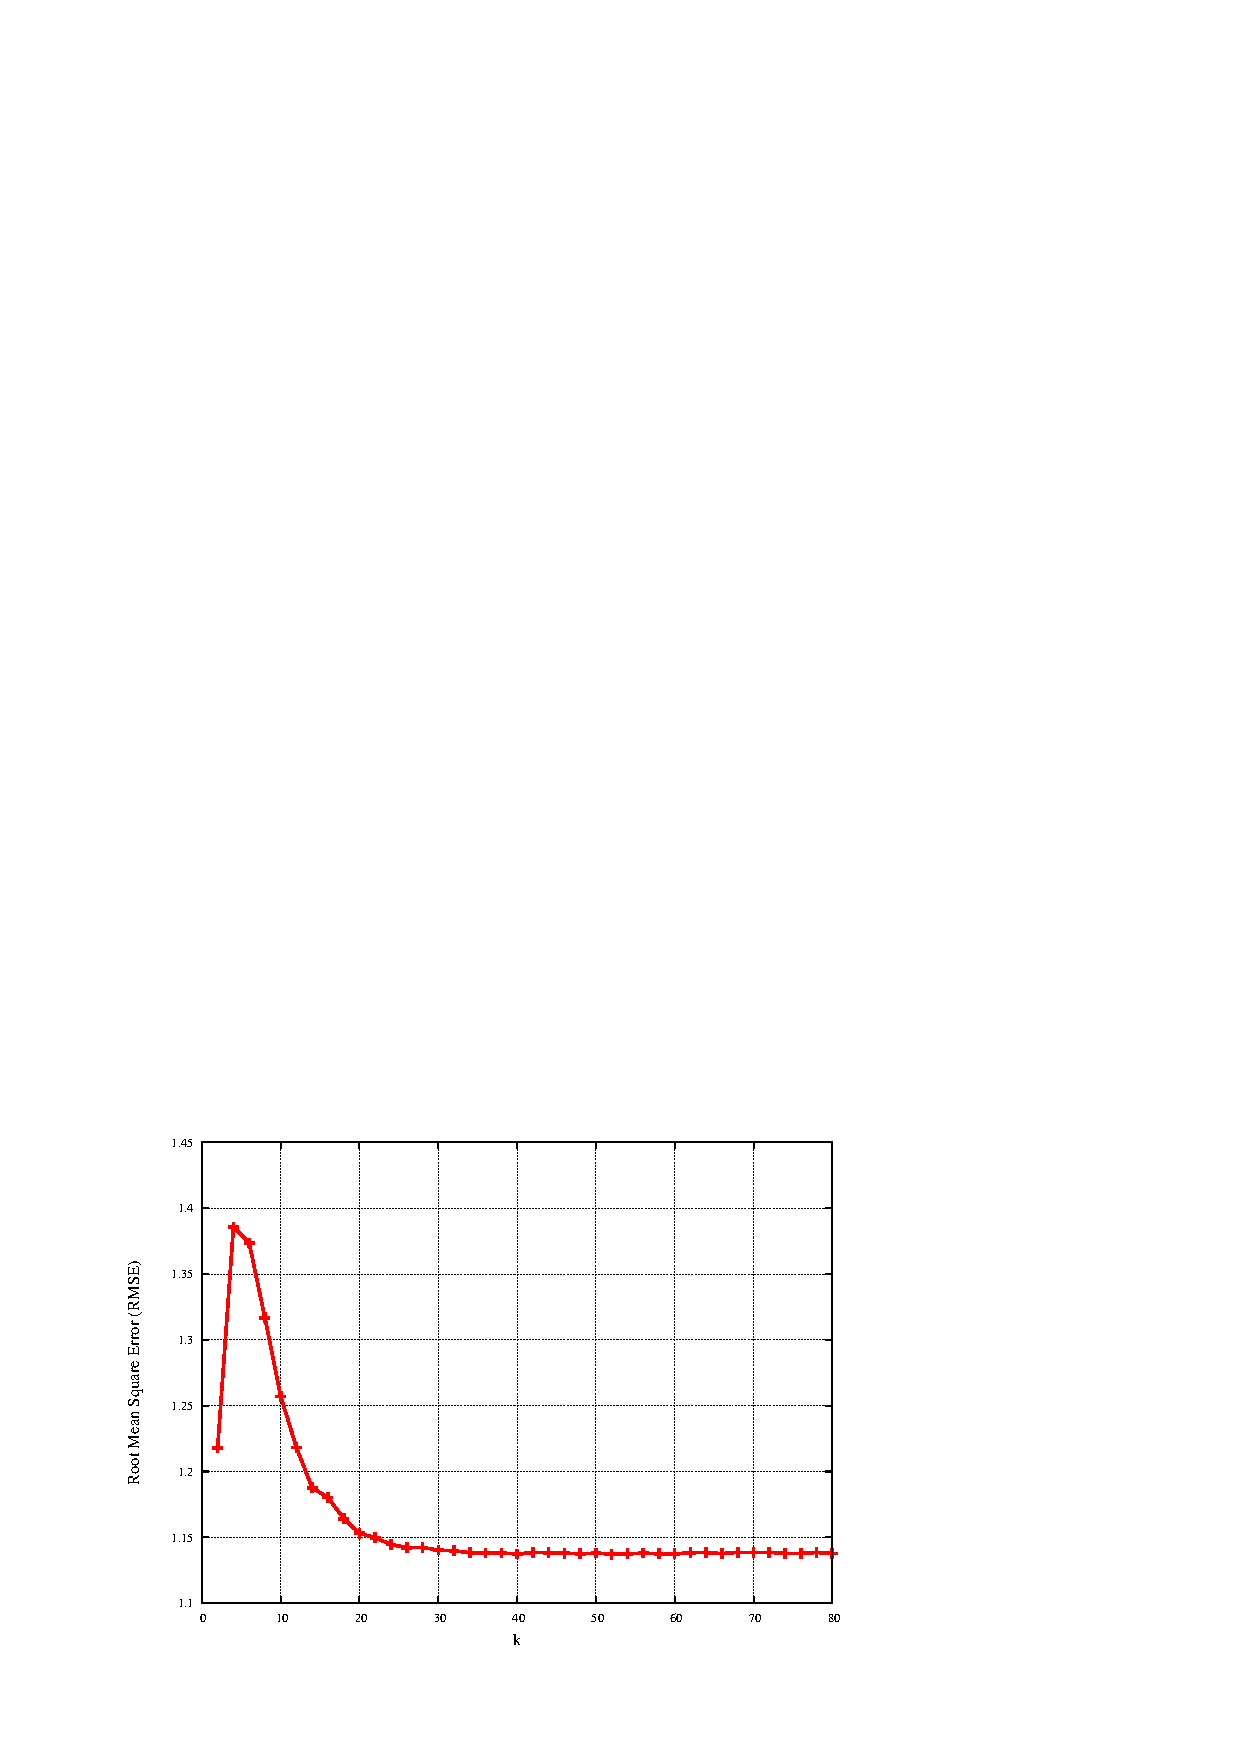
\includegraphics[scale=0.5]{figures/nocalnonorm.pdf}
%	\caption[]{A plot of RMSE vs. K for all ratings excluding 
%California businesses without normalization}
%	\label{fig:norm}
%\end{figure}

%\begin{figure}[ht!]
%	\centering
%	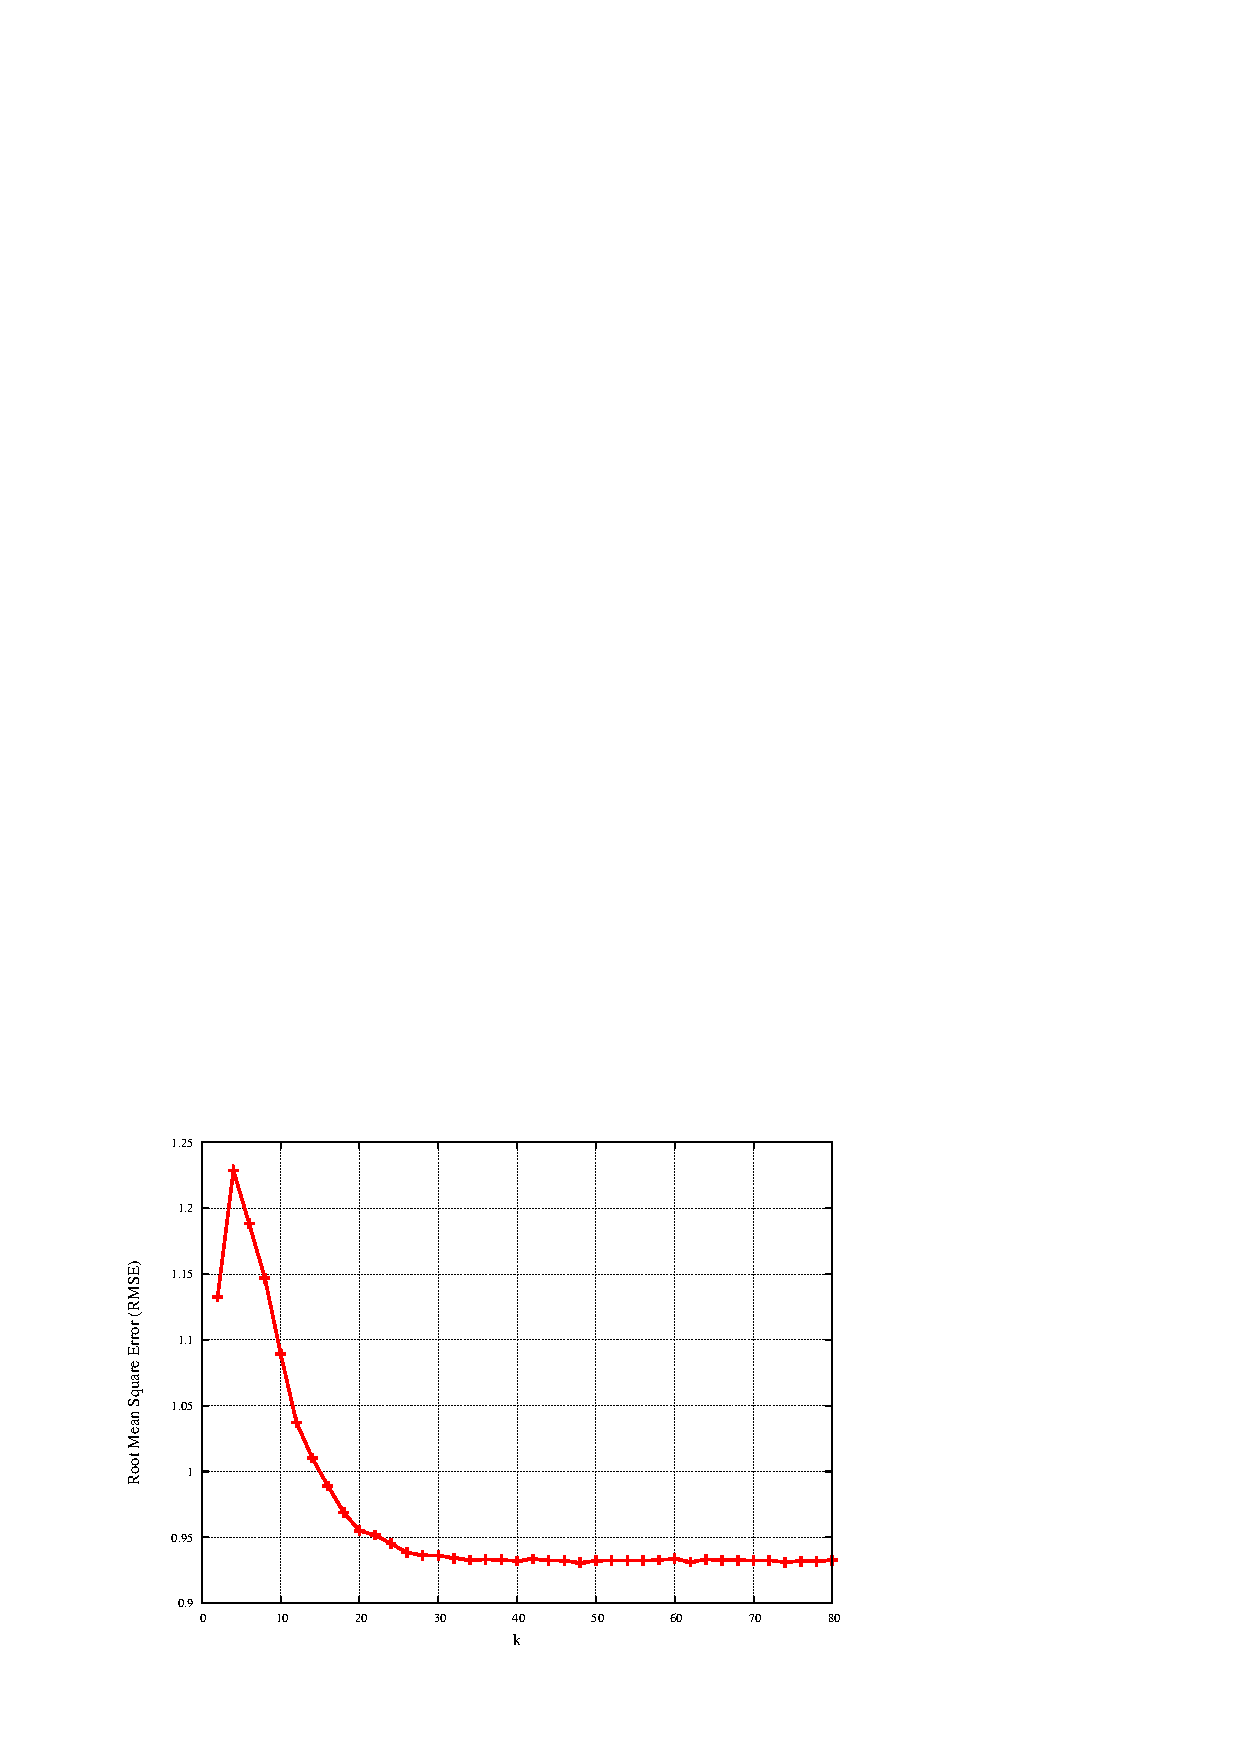
\includegraphics[scale=0.5]{figures/nocalfood.pdf}
%	\caption[]{A plot of RMSE vs. K for all food ratings excluding California businesses}
%	\label{fig:foodonly}
%\end{figure}

We also evaluated the effect of normalization by running the same tests as
above on businesses excluding California with and without a normalization
factor. Figure~\ref{fig:nocal} shows this comparison.

\subsection{Interpreting Results}
As we increase the K-values, the RMSE value approaches a minimum value which it
hovers around. For us, we were able to achieve an RMSE of \bestRMSE when
K=\bestK.
What's particularly interesting about our result is that it shows predictions
across a wide variety of businesses-genres can be useful in predicting
interests in unrelated genres. For example, predictions for clothing shops can
be used to help predict where you might like to go out to eat. We initially
thought that using unrelated businesses to predict one another would yield to
inaccurate results. However, when we excluded non-food related ratings from the
dataset, we achieved worse RMSE results. Figure~\ref{fig:cal} shows this comparison.

We also compared our results to the winners of the Netflix prize,
\cite{netprize}. Unlike our technique, the winners of the Netflix prize used a
combination of different predictors working in unison to build a prediction
engine. Ideally, we would build additional prediction engines to supplement
ours. However, we were not able to do this due to time constraints. Overall,
the winners of the Netflix prize achieved an RMSE value of \bestNetflixRMSEnsp,
which is roughly \netDiff from our best RMSE of \bestRMSEnsp. The difference
between the accuracy of our results and the Netflix results is likely due to
the fact that movies are much more controlled than businesses. Businesses are
affected by location, price, quality of service, and hours of operation. Movies
are always available and are displayed in a roughly uniform way. 




\section{Error Analysis}
Error analysis to go in here


\begin{thebibliography}{9}

\bibitem{netprize}
  Edwin Chen,
  \emph{Winning the Netflix Prize: A Summary}.
  http://blog.echen.me/2011/10/24/winning-the-netflix-prize-a-summary/
\end{thebibliography}
\end{document}
